\def\year{2019}\relax
%File: formatting-instruction.tex
\documentclass[letterpaper]{article} % DO NOT CHANGE THIS
\usepackage{aaai19}  % DO NOT CHANGE THIS
\usepackage{times}  % DO NOT CHANGE THIS
\usepackage{helvet} % DO NOT CHANGE THIS
\usepackage{courier}  % DO NOT CHANGE THIS
\usepackage[hyphens]{url}  % DO NOT CHANGE THIS
\usepackage{graphicx} % DO NOT CHANGE THIS
\urlstyle{rm} % DO NOT CHANGE THIS
\def\UrlFont{\rm}  % DO NOT CHANGE THIS
\usepackage{graphicx}  % DO NOT CHANGE THIS
\frenchspacing  % DO NOT CHANGE THIS
\setlength{\pdfpagewidth}{8.5in}  % DO NOT CHANGE THIS
\setlength{\pdfpageheight}{11in}  % DO NOT CHANGE THIS
%PDF Info Is REQUIRED.
% For /Author, add all authors within the parentheses, separated by commas. No accents or commands.
% For /Title, add Title in Mixed Case. No accents or commands. Retain the parentheses.
\usepackage{mathtools}
\usepackage{float}

 \pdfinfo{
/Title (AAAI Press Formatting Instructions for Authors Using LaTeX -- A Guide)
/Author (AAAI Press Staff, Pater Patel Schneider, Sunil Issar, J. Scott Penberthy, George Ferguson, Hans Guesgen)
} %Leave this	
% /Title ()
% Put your actual complete title (no codes, scripts, shortcuts, or LaTeX commands) within the parentheses in mixed case
% Leave the space between \Title and the beginning parenthesis alone
% /Author ()
% Put your actual complete list of authors (no codes, scripts, shortcuts, or LaTeX commands) within the parentheses in mixed case. 
% Each author should be only by a comma. If the name contains accents, remove them. If there are any LaTeX commands, 
% remove them. 

% DISALLOWED PACKAGES
% \usepackage{authblk} -- This package is specifically forbidden
% \usepackage{balance} -- This package is specifically forbidden
% \usepackage{caption} -- This package is specifically forbidden
% \usepackage{color (if used in text)
% \usepackage{CJK} -- This package is specifically forbidden
% \usepackage{float} -- This package is specifically forbidden
% \usepackage{flushend} -- This package is specifically forbidden
% \usepackage{fontenc} -- This package is specifically forbidden
% \usepackage{fullpage} -- This package is specifically forbidden
% \usepackage{geometry} -- This package is specifically forbidden
% \usepackage{grffile} -- This package is specifically forbidden
% \usepackage{hyperref} -- This package is specifically forbidden
% \usepackage{navigator} -- This package is specifically forbidden
% (or any other package that embeds links such as navigator or hyperref)
% \indentfirst} -- This package is specifically forbidden
% \layout} -- This package is specifically forbidden
% \multicol} -- This package is specifically forbidden
% \nameref} -- This package is specifically forbidden
% \natbib} -- This package is specifically forbidden -- use the following workaround:
% \usepackage{savetrees} -- This package is specifically forbidden
% \usepackage{setspace} -- This package is specifically forbidden
% \usepackage{stfloats} -- This package is specifically forbidden
% \usepackage{tabu} -- This package is specifically forbidden
% \usepackage{titlesec} -- This package is specifically forbidden
% \usepackage{tocbibind} -- This package is specifically forbidden
% \usepackage{ulem} -- This package is specifically forbidden
% \usepackage{wrapfig} -- This package is specifically forbidden
% DISALLOWED COMMANDS
% \nocopyright -- Your paper will not be published if you use this command
% \addtolength -- This command may not be used
% \balance -- This command may not be used
% \baselinestretch -- Your paper will not be published if you use this command
% \clearpage -- No page breaks of any kind may be used for the final version of your paper
% \columnsep -- This command may not be used
% \newpage -- No page breaks of any kind may be used for the final version of your paper
% \pagebreak -- No page breaks of any kind may be used for the final version of your paperr
% \pagestyle -- This command may not be used
% \tiny -- This is not an acceptable font size.
% \vspace{- -- No negative value may be used in proximity of a caption, figure, table, section, subsection, subsubsection, or reference
% \vskip{- -- No negative value may be used to alter spacing above or below a caption, figure, table, section, subsection, subsubsection, or reference

\setcounter{secnumdepth}{0} %May be changed to 1 or 2 if section numbers are desired.

% The file aaai19.sty is the style file for AAAI Press 
% proceedings, working notes, and technical reports.
%
\setlength\titlebox{2.5in} % If your paper contains an overfull \vbox too high warning at the beginning of the document, use this
% command to correct it. You may not alter the value below 2.5 in
\title{Visionary: Voice Guide for Visually Handicapped People  \\--- CS3244 Group 26 Project }
%Your title must be in mixed case, not sentence case. 
% That means all verbs (including short verbs like be, is, using,and go), 
% nouns, adverbs, adjectives should be capitalized, including both words in hyphenated terms, while
% articles, conjunctions, and prepositions are lower case unless they
% directly follow a colon or long dash
\author{\Large \textbf{Jin Shuyuan$\thanks{All of us contributed equally}$ , Mou Ziyang$^{*}$, Tian Xin$^{*}$}\\ \Large \textbf{Tian Xueyan$^{*}$, Wang Tengda$^{*}$, Zhao Tianze$^{*}$}\\ % All authors must be in the same font size and format. Use \Large and \textbf to achieve this result when breaking a line
%If you have multiple authors and multiple affiliations
% use superscripts in text and roman font to identify them. For example, Sunil Issar,\textsuperscript{\rm 2} J. Scott Penberthy\textsuperscript{\rm 3} George Ferguson,\textsuperscript{\rm 4} Hans Guesgen\textsuperscript{\rm 5}. Note that the comma should be placed BEFORE the superscript for optimum readability
National University of Singapore\\
shuyuanjin@u.nus.edu(A0162475B), ziyang.mou@u.nus.edu(A0147984L), tian.xin@u.nus.edu(A0148036H),\\
tian.xueyan@u.nus.edu(A0177357R), tengda@u.nus.edu(A0177660X), zhao.tianze@u.nus.edu(A0147989B)\\ % email address must be in roman Bext type, not monospace or sans serif
}
\pagestyle{plain}
\begin{document}

\maketitle

\begin{abstract}
This paper presents our idea of the app: \textit{Visionary}. \textit{Visionary} is a voice guide app for visually handicapped people to assist them in avoiding approaching people on the street. With the help of the phone camera, \textit{Visionary} can capture real-time scenes in front of the user, classify objects and make voice warning to inform the user that some people are approaching. Our app adopts a state-of-the-art object detection Machine Learning model called YOLOv3 whose structure and algorithm are explained in YOLOv3 section. To determine other pedestrians moving direction and output audio, bounding boxes sizes are compared and CMU Flite Text-to-Speech Synthesis Engine is utilized. Additionally, some other plausible Machine Learning algorithms and their comparisons to YOLOv3 are shown in other Machine Learning Methods part. We believe \textit{Visionary} will have an extensive impact on the lives of visually handicapped people and their family in Singapore. 
\end{abstract}

\section{Background}

As of March 2017, the population of low-vision and blind residents registered to Singapore Association of the Visually Handicapped is 3814\cite{savh-data}. The Singapore government has built tactile paving in all the subway stations and most of the walking paths for visually handicapped people. For those who would like to walk on the tactile paving, in-door and out-door walking guide system based on GPS could be easily built for them, the correct route could be feedback to the visually handicapped user to ensure they are heading the correct direction. However, in this case, other pedestrians become one of the most critical uncertainty - they are not predictable. If a pedestrian does not notice the visually handicapped user, they may walk into each other which may cause severe consequences and is pretty dangerous. \\

\noindent We have implemented a system to detect approaching pedestrians with Machine Learning and translate the information to voice (Fig.~\ref{fig:demo}). Our product will act as an add-on system for the guide system for visually handicapped users to feedback real-time walking guide. With the help of our system, the blind users will be able to get more real-time conditions about the path ahead so that they can avoid danger caused by approaching pedestrians. \textit{Visionary} will help them walk faster and walk safer, improving their life quality.
%%%%%%%%%%%%%%%%%%%%%%%%%%%%%%%%%%%%%%%%%%%%%%%%%%%%%%%%
\begin{figure}[ht]
\hspace{0mm}
\centering
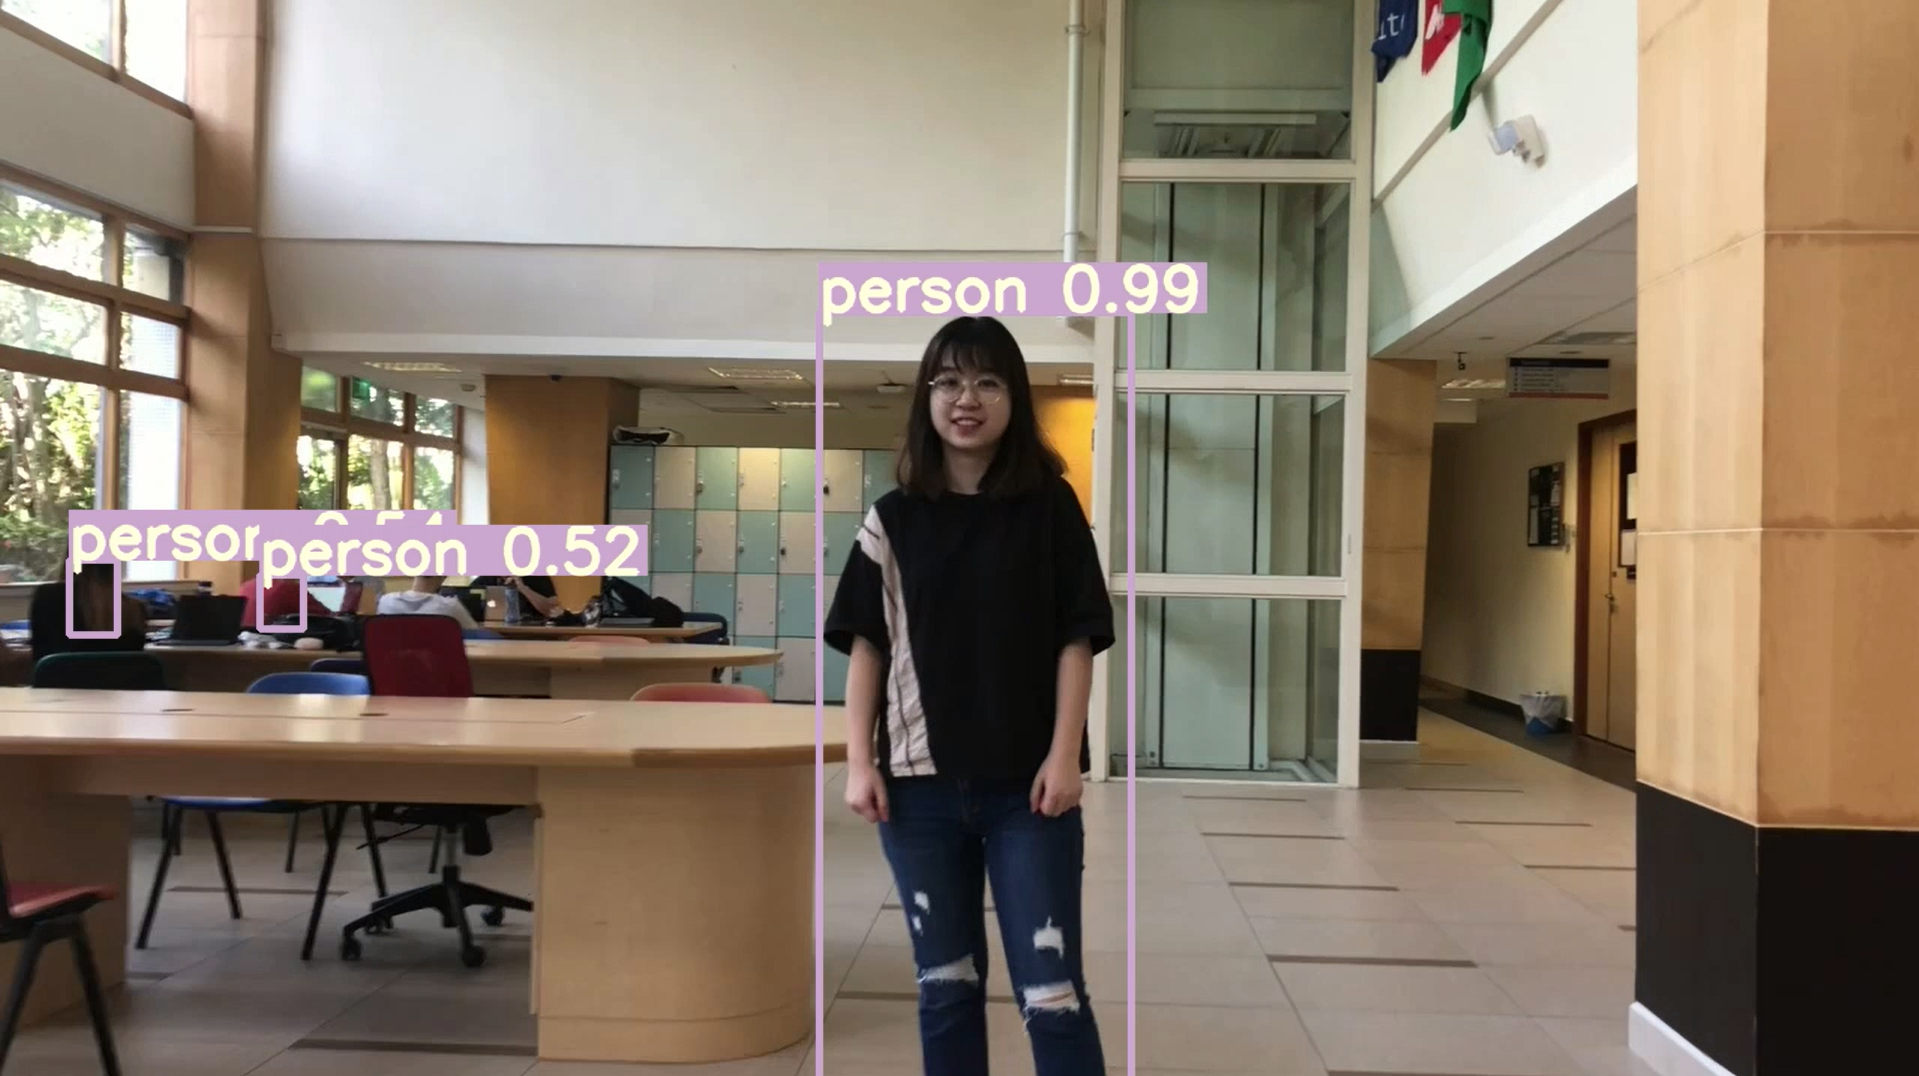
\includegraphics[width=0.85\linewidth,height = 0.5\linewidth]{Figure/demo1.png}
\caption{\footnotesize{Demonstration result.}}
\label{fig:demo}
\vspace{0mm}
\end{figure}
%%%%%%%%%%%%%%%%%%%%%%%%%%%%%%%%%%%%%%%%%%%%%%%%


\section{App Implementations}
\textit{Visionary} takes sequential RGB images or video as input and outputs voice reminders for whether there exist any approaching pedestrians.
\begin{itemize}
\item The input accepts three formats: image series, videos and real-time webcam images.
\item The output is a voice guide. When other people are moving towards the user, \textit{Visionary} will say "Approaching". Otherwise, our app will not make any voice output. Apart from audio, images and videos with bounding boxes and type labels are also available for reference(Fig.\ref{fig:demo}). 
\end{itemize}

\noindent The code implementation can be found in our Github repository\footnote{https://github.com/CoderStellaJ/CS3244-ML-Project}. We choose YOLOv3 as our Machine Learning method to detect pedestrians. This Machine Learning algorithm can detect human objects within a short time period and achieve high accuracy, which is important for a real-time guide system. The pedestrians in input video could be detected correctly without any limitation of video shooting direction, which is a must for our product because pedestrians may come from all directions (Fig.~\ref{fig:arc}). \\

\noindent Other than the YOLOv3 model, we design and implement an algorithm to detect objects moving direction. This algorithm compares the bounding box size in the current frame with the average size of the previous five frames. For each of the frame, we find the largest bounding box because we consider it as the nearest person to the user. If either width or height of the bounding box is larger than the average of previous 5 frames, we assume the object is approaching the user. We design this algorithm because the camera may not always capture a full-size human. During our experiments, when the user is approaching another pedestrian, the area of the bounding box may decrease because the legs of the pedestrian are not within the camera's angle of view. However, in this case, the width of the bounding box still increases. Thus comparing box width or height is more reasonable and works better. \\

\noindent After comparing different ways of transforming text message to sound, we adopt CMU Flite Text-to-Speech Synthesis Engine to generate our sound files based on the text in our final implementation. Those sound files are played to notify the user if \textit{Visionary} predicts someone is approaching. 
%%%%%%%%%%%%%%%%%%%%%%%%%%%%%%%%%%%%%%%%%%%%%%%%
\begin{figure}[ht]
\hspace{-6mm}
\centering
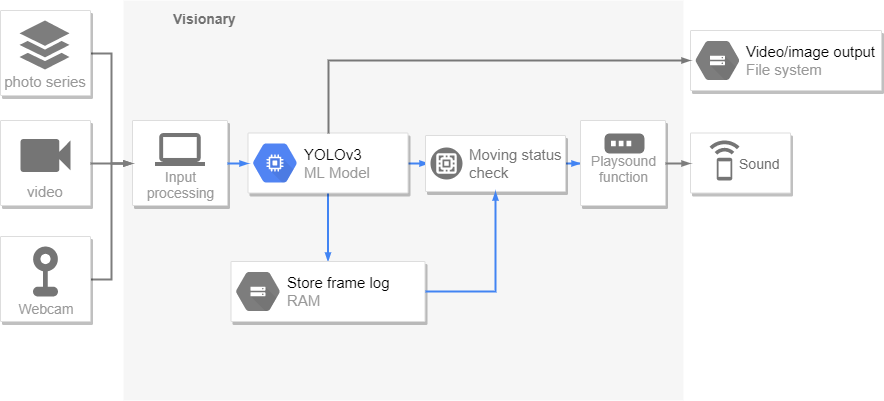
\includegraphics[width=1.1\linewidth,height = 0.5\linewidth]{Figure/Code_structure_diagram.png}
\caption{\footnotesize{System architecture}}
\label{fig:arc}
\vspace{-2mm}
\end{figure}
%%%%%%%%%%%%%%%%%%%%%%%%%%%%%%%%%%%%%%%%%%%%%%%%

\subsection{App Features}
\begin{itemize}
\item Camera based image capturing \\
Open webcam to capture real-time view in front of the user as input.
\item Object detection and classification \\
Use our Machine Learning model to detect the person object in input stream.
\item Moving direction determination \\
Based on person object detected from input images, we design a direction determination algorithm to determine whether the pedestrian in front is approaching the user and may cause danger.
\item Voice Guide \\
Based on object classification and moving direction, output voice guide (any pedestrian approaching)
\end{itemize}
\subsection{App Algorithm Requirements}
In order to achieve our goal to help blind people navigate around, our app algorithm needs to model human visual system. Human eyes can capture real-time scenes constantly for a long period of time and the visual system is fast and accurate in detecting objects in scenes, classifying them and estimating their moving directions. Equipped with this ability, humans are able to make proper decisions such as stopping or changing direction to avoid obstacles. However, for detection systems, there is always a trade-off between accuracy and speed. We want neither a highly accurate but over-complex slow model nor a fast but error-prone method. Thus, the chosen machine learning algorithm should satisfy the following requirements:
\begin{itemize}
    \item Continuously take sequential images or videos as input and generate real-time outputs consisting of object detection and classification.
    \item Keep a good balance between speed and accuracy when performing the task.
\end{itemize}
Based on the above requirements, we finally chose YOLOv3\cite{YOLO} as the core machine learning part of our app. Compared with other Machine Learning detection systems, YOLOv3 can realize real-time detection and in the meanwhile keep relatively high Mean Average Precision(mAP)\cite{YOLO}. More details of qualitative and quantitative comparisons can be found in Other Methods and Experiments and Results section.

\section{YOLOv3}
You Only Look Once(YOLO) was first introduced by \cite{YOLO}. After that, YOLO has been improved over the years and the latest version is YOLOv3\cite{YOLOv3}. In this section, we will take a closer look at its technical details.
%%%%%%%%%%%%%%%%%%%%%%%%%%%%%%%%%%%%%%%%%%%%%%%%%%%%%%%%
\begin{figure}[ht]
\hspace{-6mm}
\centering
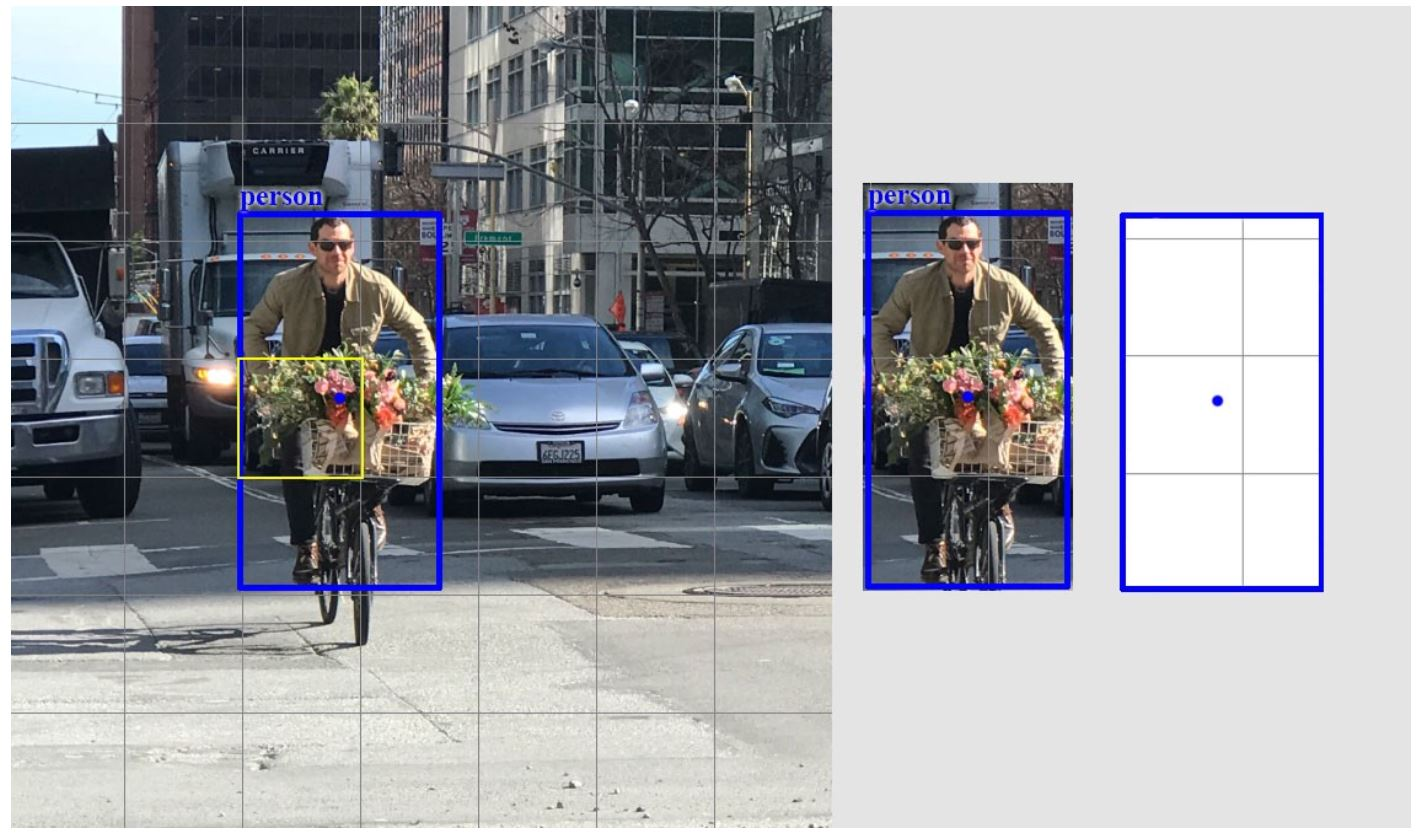
\includegraphics[width=0.85\linewidth,height = 0.5\linewidth]{Figure/gridcells.JPG}
\caption{\footnotesize{YOLOv3 divides an image into $N*N$ grid cells.}}
\label{fig:cells}
\vspace{-2mm}
\end{figure}
%%%%%%%%%%%%%%%%%%%%%%%%%%%%%%%%%%%%%%%%%%%%%%%%
\subsection{Grid Cell}
YOLOv3 divides the image into $N*N$ grid cells. Each cell draws B bounding boxes at different scales and classifies object type inside each box (Fig.~\ref{fig:cells}). Every bounding box consists of the following parameters:
\begin{itemize}
    \item $t_x$, $t_y$, $t_w$ and $t_h$, which are related to the coordinates of the box's center as well as the width and height of the box.
    \item The probability that the box contains an object $P(Object)$, which is called objectness.
    \item Class scores $P(Class_{i}|Object)$ for C class types.
\end{itemize}
The final prediction of YOLOv3 is encoded as a $N*N*(B*(4+1+C))$ tensor.

%%%%%%%%%%%%%%%%%%%%%%%%%%%%%%%%%%%%%%%%%%%%%%%%%%
\begin{figure}[ht]
\hspace{-6mm}
\centering
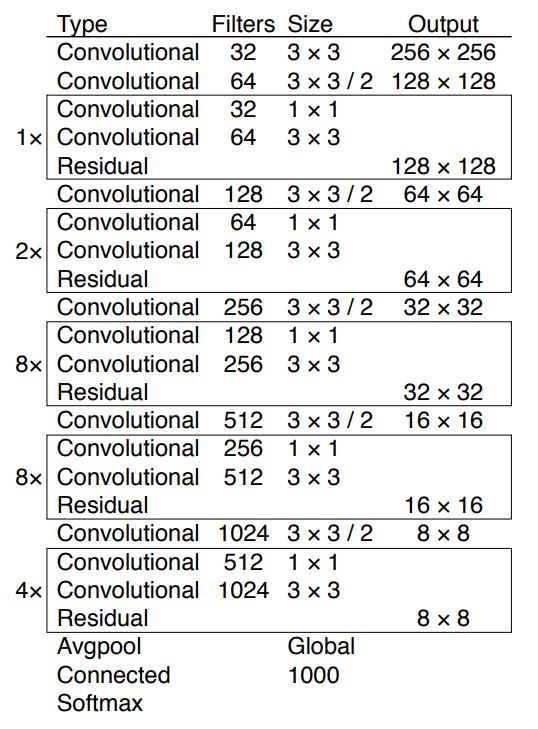
\includegraphics[width=0.85\linewidth,height = 1\linewidth]{Figure/yolov3_structure.JPG}
\caption{\footnotesize{YOLOv3 network for feature extraction.}}
\label{fig:network}
\vspace{-2mm}
\end{figure}
%%%%%%%%%%%%%%%%%%%%%%%%%%%%%%%%%%%%%%%%%%%%%%

\subsection{Network Design}
As shown in Fig.~\ref{fig:network}, a CNN with 53 layers is used to perform feature extraction from images. The features are then fed into a regression to make predictions. 

\subsection{Loss Function}
The loss function of YOLOv3 consists of:
\begin{itemize}
    \item Localization Loss\\
    The localization loss measures the errors in the location and size of the predicted boundary box.
\begin{equation}
\begin{aligned}
loss_{loc} = \lambda_{loc}*(MSE(x, \hat{x})+MSE(y, \hat{y})\\+MSE(w, \hat{w})+MSE(h, \hat{h}))
\end{aligned}
\end{equation}
\scriptsize
where MSE is mean squared error
\normalsize
 \item Objectness Loss\\
    The objectness loss measures the error in predicting whether a bounding box contains objects.
    \begin{equation}
   loss_{obj} = \lambda_{obj}*BCE(P(Object), \hat{Object})
   \end{equation}
   \scriptsize
where BCE is binary cross-entropy
\normalsize

    \item Classification Loss\\
    The classification loss reflects the accuracy of classifying the correct object type given the object in the box.
    \begin{equation}
    loss_{class} = \lambda_{class}*CE(P(Class_{i}|Object), \hat{Class_i})
    \end{equation}
    \scriptsize
where CE is cross-entropy
\normalsize
\end{itemize}
The final multi-part loss for YOLOv3 neural network is:
\begin{equation}
loss_{final} = loss_{loc} + loss_{obj} + loss_{class}
\end{equation}


%%%%%%%%%%%%%%%%%%%%%%%%%%%%%%%%%%%%%%%%%%%%%%%%%%%
\begin{figure}[ht]
\hspace{-10mm}
\centering
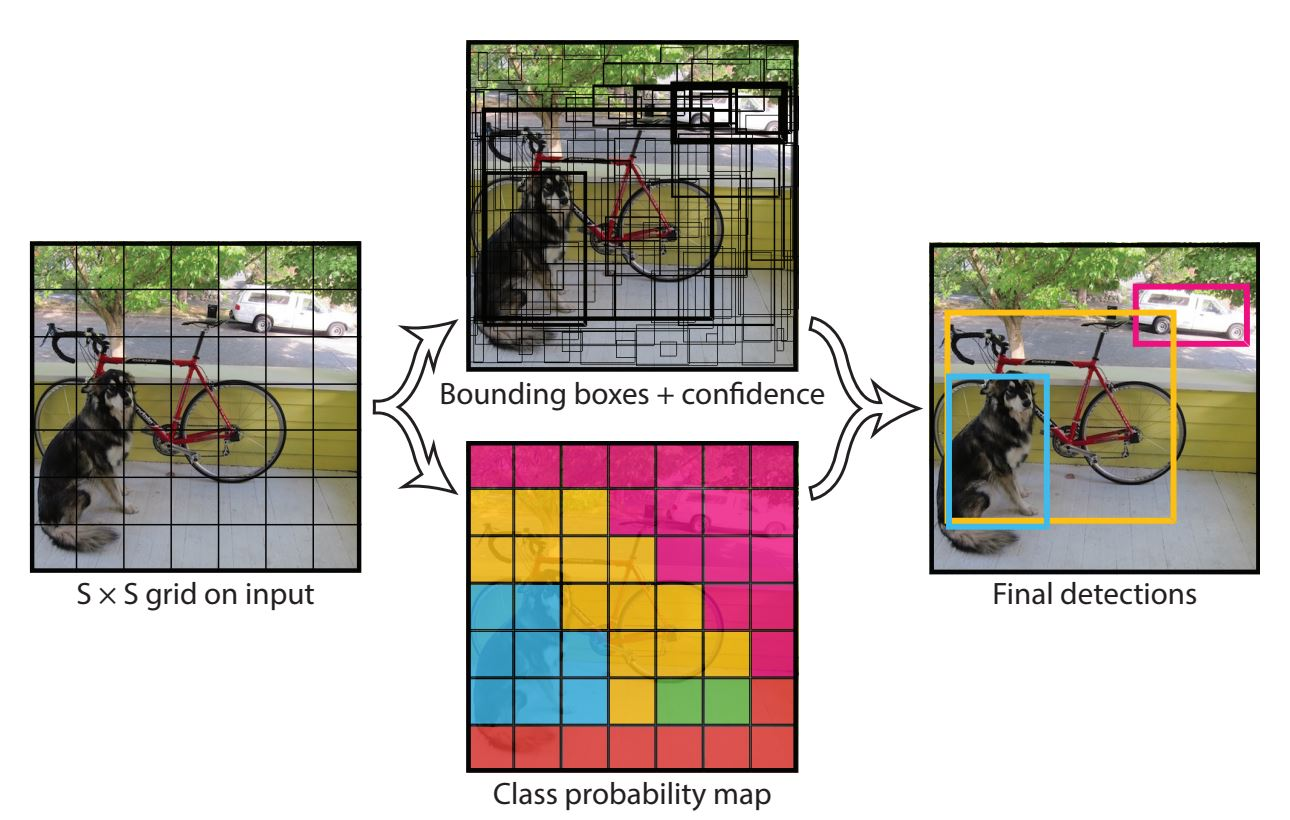
\includegraphics[width=0.85\linewidth,height = 0.5\linewidth]{Figure/yolo_grid.JPG}
\caption{\footnotesize{YOLOv3 system working process.}}
\label{fig:grid}
\vspace{-2mm}
\end{figure}
%%%%%%%%%%%%%%%%%%%%%%%%%%%%%%%%%%%%%%%%%%%%%%%%%%%%%
\subsection{Inference}
At this inference stage, final class-specific confidence for each bounding box is computed(Fig.~\ref{fig:grid}):
\begin{equation}
    conf_{class} = P(Class_{i}|Object)*P(Object) = P(Class_{i})
\end{equation}

\noindent To make sure that one object is bounded by exactly one box, \cite{YOLOv3} uses non-maximal suppression. Here is its implementation\cite{YOLOslides}:
\begin{itemize}
    \item Sort the predictions by the class-specific confidence scores.
    \item Start from the prediction with the highest score, ignore or remove any current prediction if there exists a previous prediction that has the same class label and $IoU\footnote{IOU is union intersection between ground truth and predicted bounding box}$ $>$ 0.5 with the current prediction.
    \item Repeat the previous step until all predictions are checked.
\end{itemize}

\subsection{Interesting Behavior of YOLOv3}
YOLOv3 is extremely fast. \cite{YOLOv3} designs the model as a unified single neural network whose performance can be optimized end-to-end directly instead of a complicated pipeline. During prediction, the bounding box coordinates and class probabilities straightly come from image pixels where we look at the image only once.\\

\noindent Previous region-proposal methods limit the classifier to some specific regions. Compared with them, YOLOv3 accesses to the whole image so that it demonstrates fewer background errors during prediction.\\

\noindent Most object detection systems assume that class labels are mutually exclusive. However, in reality, a "pedestrian" could also be a "child". In YOLOv3, logistic classifiers replace softmax function used in other systems so that all class scores $P(Class_{i}|Object)$ don't necessarily sum up to 1 and an object can be multi-labeled\cite{YOLOdev}.

\subsection{YOLOv3 and Our App}
Based on assessment of several existing object detecting models, we decided to use YOLOv3, as it generally net our expectations and fit the requirement of our proposed application best.\\
\\
\noindent YOLOv3 is fast. It runs significantly faster than other detection methods with comparable performance. Therefore, it can render real-time object recognition and classification, which is extremely significant in assisting visually impaired people to observe the surroundings. It balances speed and accuracy performance. In our application, since we are only detecting real-world moving human objects, speed dominates performance, and obviously YOLOv3 is the model that excels the others. In terms of detecting objects, YOLOv3 is doing well comparing its performance with human eyes. YOLOv3 is strong in a detection metric of mAP at IOU=0.5. Yet, according to \cite{Human-machine}, it is difficult for even human beings to distinguish a bounding box with IOU of 0.3 from one with IOU 0.5. Hence it is sufficient for YOLOv3 to work with IOU=0.5 and accurately detecting neighboring objects for visually handicapped people.\\

\noindent YOLOv3 reasons globally about the image when making predictions\cite{YOLOv3}. Since we are detecting the person with the closest distance to the user, it is good to have a comprehensive overview of the surroundings. It is also easily extensible, as we can further predict objects other than persons in the same frame. Furthermore, it is good that YOLOv3 learns generalizable representations of objects, so it is less likely to break down when applied to new domains or unexpected input given the unpredictable nature of the surrounding environment. \cite{YOLOv3} However, due to hardware limitations, we are not able to produce ideal outputs using our own laptops and phones although the model is theoretically competitive.

\subsection{Improvements on Current Model}
Since our app cares about only the human object closest to the user, there might be inconsistency in the assumption if YOLOv3 uses bounding box. For instance, a person stretching his arms might be more distant but has larger bounding box size than a nearer person standing straight. In order to cope with this issue, alternatives to bounding box method could be attempted. A new approach called Mask R-CNN was proposed by \cite{Mask-RCNN}, which predicts an object mask in parallel with bounding box. Incorporating object mask in the current model would effectively reduce the probability of making wrong assumption, and hence improve application performance.

\section{Other Machine Learning Methods}
This section describes other possible methods and compares them with YOLOv3.

\subsection{R-CNN}
As shown in Fig.~\ref{fig:r_cnn}, R-CNN performs selective search \footnote{Selective Search is a region proposal algorithm that generates hierarchical grouping of similar regions in terms of color, texture, size and shape compatibility.} on the input images and extracts 2000 bottom-up region proposals. These 2000 candidates are fed into a large convolutional neural network(CNN) that outputs a 4096-dimensional feature vector. The extracted features are fed into an SVM \footnote{Support Vector Machine is a supervised learning method that looks at data and sorts it into one of two categories} to classify the presence of the object within that region proposal. Post-processing is used to refine the bounding boxes and eliminate duplicate detections.\\

\noindent Although R-CNN achieves a mean average precision(mAP) of 53.7\% on PASCAL VOC 2010, the model needs to examine 2000 region proposals and spends around 47s on each test image. Therefore, R-CNN cannot be implemented real-time.
%%%%%%%%%%%%%%%%%%%%%%%%%%%%%%%%%%%%%%%%%%%%%%%%%%%
\begin{figure}[ht]
\hspace{0mm}
\centering
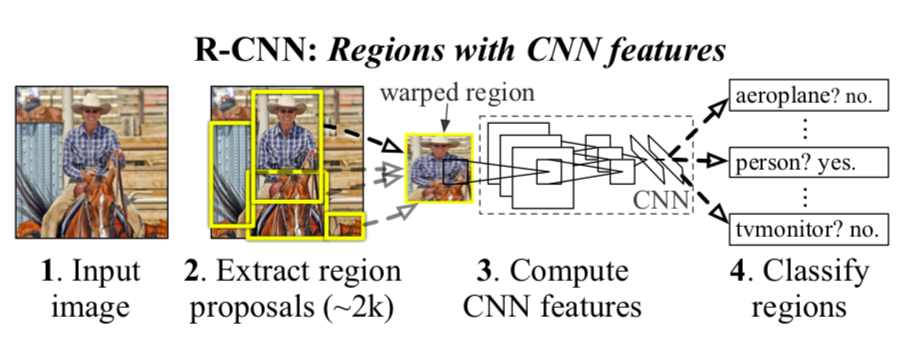
\includegraphics[scale = 0.28]{Figure/r_cnn.png}
\caption{\footnotesize{Architecture of R-CNN.}}
\label{fig:r_cnn}
\vspace{0mm}
\end{figure}
%%%%%%%%%%%%%%%%%%%%%%%%%%%%%%%%%%%%%%%%%%%%%%%%%%%%%
\subsection{Fast R-CNN}
According to Fig.~\ref{fig:fast_2}, Fast R-CNN fits the entire image into a fully convolutional neural network to generate a feature map. It then performs selective search algorithm on the feature map to identify region proposals and uses RoI pooling\footnote{A pooling layer which performs max pooling on inputs of non-uniform sizes and produces a small feature map of fixed size.} layer to reshape them into the required size. The network has two output vectors per RoI: namely softmax probabilities and per-class bounding-box regression offsets.\\

\noindent By experiment, although Fast R-CNN offers speed and accuracy improvement over R-CNN, it still falls short of real-time detection.
%%%%%%%%%%%%%%%%%%%%%%%%%%%%%%%%%%%%%%%%%%%%%%%%%%%
\begin{figure}[ht]
\hspace{0mm}
\centering
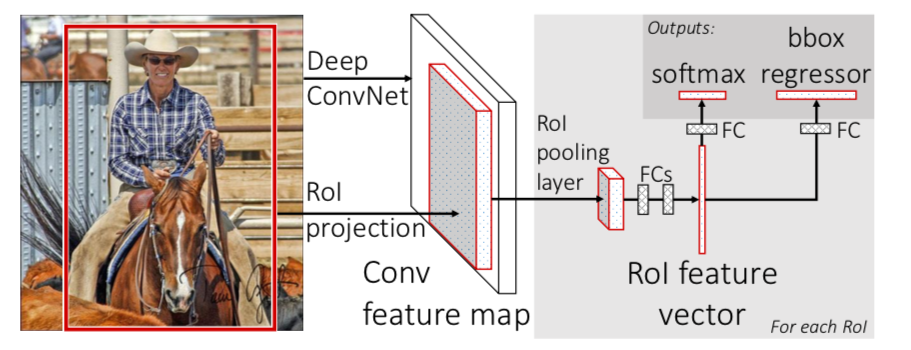
\includegraphics[scale=0.25]{Figure/fast_r_cnn.png}
\caption{\footnotesize{Work flow of Fast R-CNN. The architecture is trained end-to-end with a multi-task loss.}}
\label{fig:fast_2}
\vspace{0mm}
\end{figure}
%%%%%%%%%%%%%%%%%%%%%%%%%%%%%%%%%%%%%%%%%%%%%%%%%%%%%

% \noindent YOLO can see the whole image so its detection and classification involves contexture information.\\

\subsection{Faster R-CNN}
The distinctive difference between Faster R-CNN and Fast R-CNN is that it does not use selective search to generate region proposals. In Faster R-CNN algorithm, a region proposal network (RPN) is used to create region proposals. \cite{fasterRcnn}\\

\noindent The region proposal network is a convolutional neural network, which takes in feature map as an input. A $3 \times 3$ window with depth $K$ is slid through the feature map, outputting a vector with 256 features for each window. These features are fed into 2 fully-connected layers, box-regression layer and box-classification layer, to compute the boundary box. Then, the output region proposals are fed into the RoI pooling layer in the Fast R-CNN algorithm. (Fig.~\ref{fig:rpn})\\
%%%%%%%%%%%%%%%%%%%%%%%%%%%%%%%%%%%%%%%%%%%%%%%%%%%%%
\begin{figure}[ht]
    \hspace{-14mm}
    \centering
    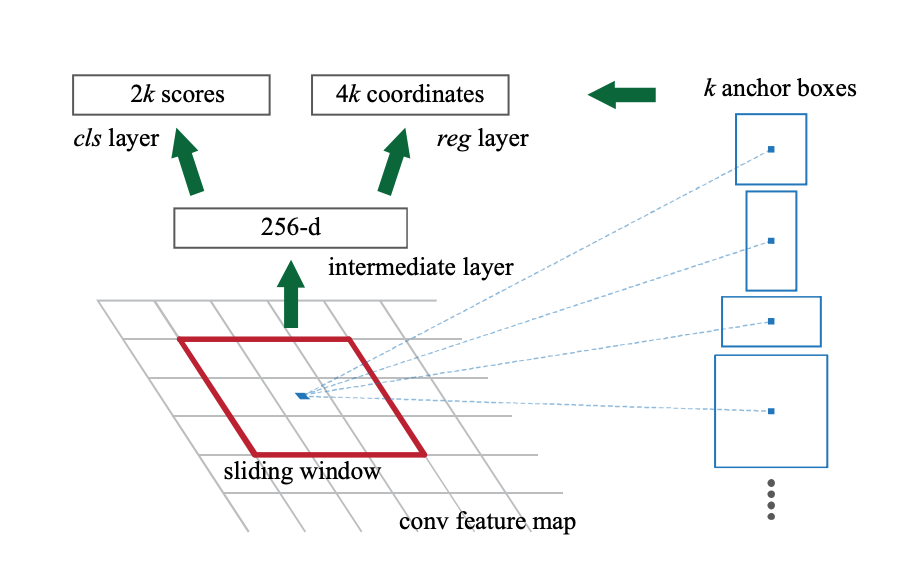
\includegraphics[width=0.85\linewidth,height = 0.55\linewidth]{Figure/faster_r_cnn.png}
    \caption{\footnotesize{Region proposal network of Faster R-CNN.}}
    \label{fig:rpn}
    \vspace{0mm}
\end{figure}
\\
%%%%%%%%%%%%%%%%%%%%%%%%%%%%%%%%%%%%%%%%%%%%%%%%%%%%%
\noindent 
Faster R-CNN reduces the object detection time to 0.2 seconds, as the time-consuming step of selective search is replaced by region proposal network. Compared to YOLOv3, it has higher correctness but longer detection time.

\subsection{Deformable Parts Model}
%%%%%%%%%%%%%%%%%%%%%%%%%%%%%%%%%%%%%%%%%%%%%%%%%%%
\begin{figure}[ht]
\hspace{-13mm}
\centering
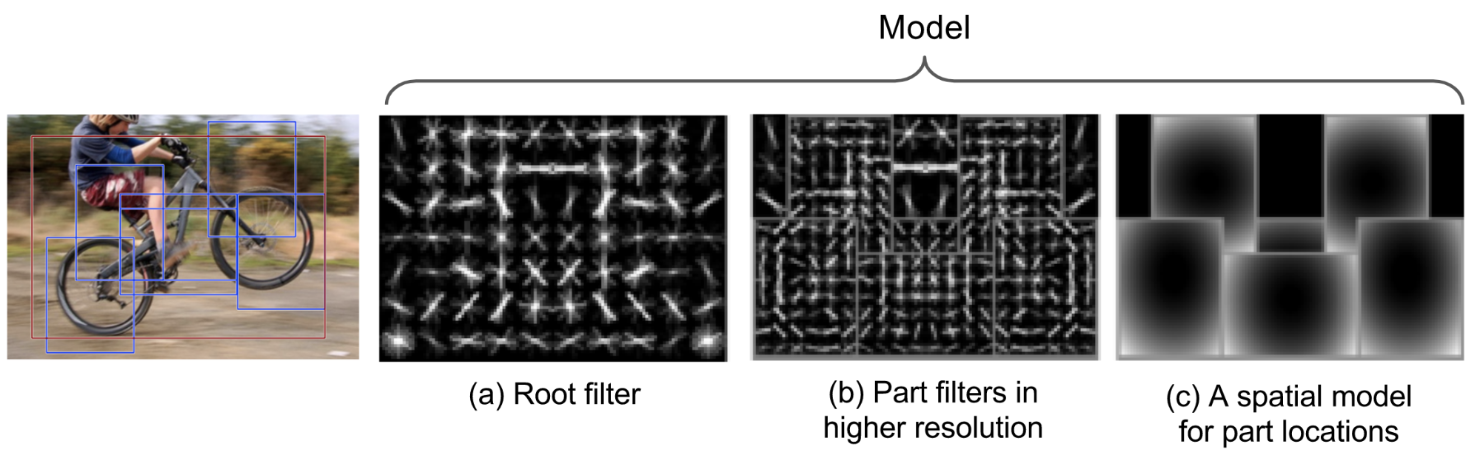
\includegraphics[width=1.0\linewidth,height = 0.3\linewidth]{Figure/DPM_1.png}
\caption{\footnotesize{Components of DPM model}}
\label{fig:DPMcomp}
\vspace{0mm}
\end{figure}
%%%%%%%%%%%%%%%%%%%%%%%%%%%%%%%%%%%%%%%%%%%%%%%%%%%%%
\noindent The Deformable parts model can detect and localize objects with a mixture of the graphical model of deformable parts\cite{DPM}. The model(Fig.~\ref{fig:DPMcomp}) contains three important components, which are root filter, part filter, and one spatial model. First, a root filter constructs a detection window that approximately covers the locations of the objects. Then, smaller parts of the object will be covered by multiple part filters. These part filters are learned at twice the resolution of the root filter. Finally, a spatial model is used to score the locations of part filters relative to the root.\\

\noindent Fig.\ref{fig:DPM_2} illustrates how DPM matching process works in details. However, the performance of DPM in some experiments(Fig.~\ref{fig:R_1}) shows that either the speed or the accuracy is worse than YOLOv3.\\
%%%%%%%%%%%%%%%%%%%%%%%%%%%%%%%%%%%%%%%%%%%%%%%%%%%
\begin{figure}[ht]
\hspace{-14mm}
\centering
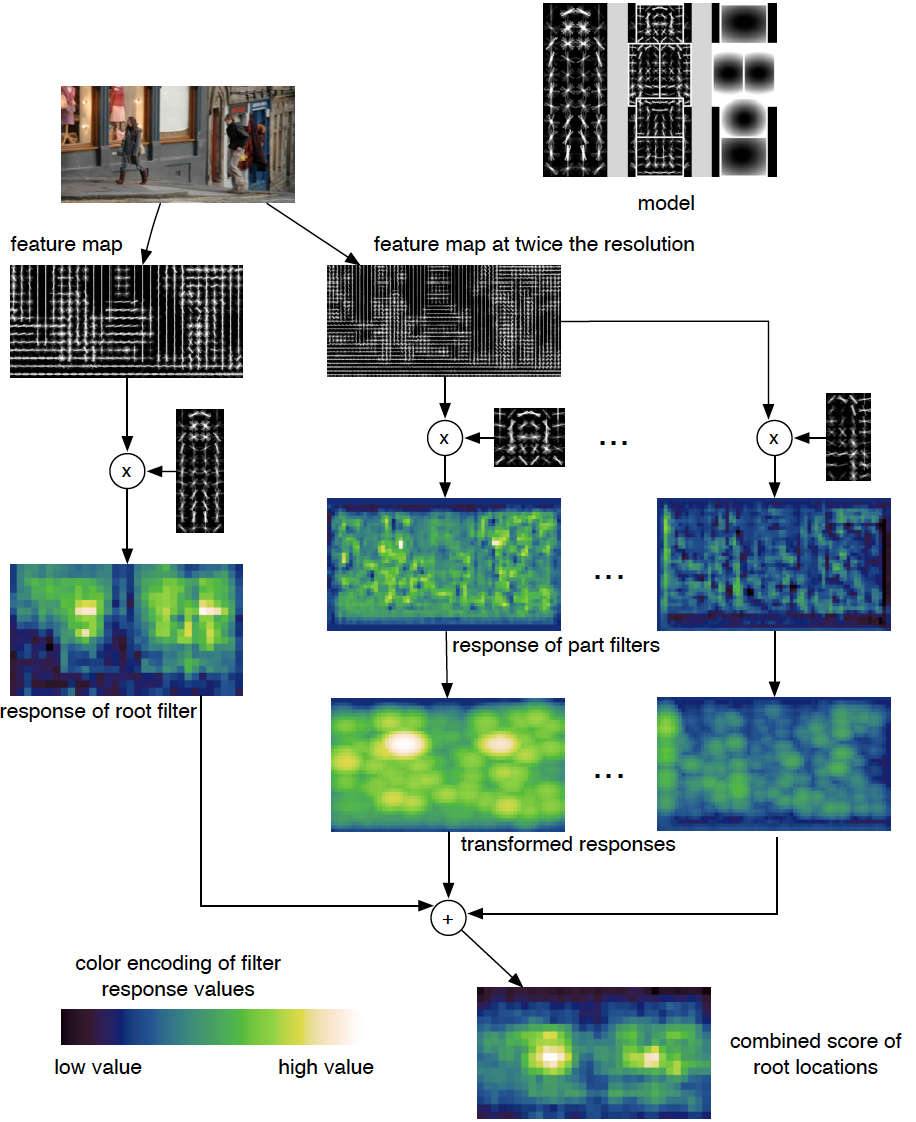
\includegraphics[width=0.85\linewidth,height = 1.0\linewidth]{Figure/DPM_2.png}
\caption{\footnotesize{DPM maching process}}
\label{fig:DPM_2}
\vspace{-3mm}
\end{figure}
%%%%%%%%%%%%%%%%%%%%%%%%%%%%%%%%%%%%%%%%%%%%%%%%%%%%

\subsection{RetinaNet}
Lin et al (\citeyear{retinaNet}) introduced RetinaNet, a one-stage detector with a new-designed focal loss as loss function, ResNet+FPN as the backbone for feature extraction, plus two task-specific sub-networks for classification and bounding box regression.\\

%%%%%%%%%%%%%%%%%%%%%%%%%%%%%%%%%%%%%%%%%%%%%%%%%%%
\begin{figure}[ht]
\hspace{-10mm}
\centering
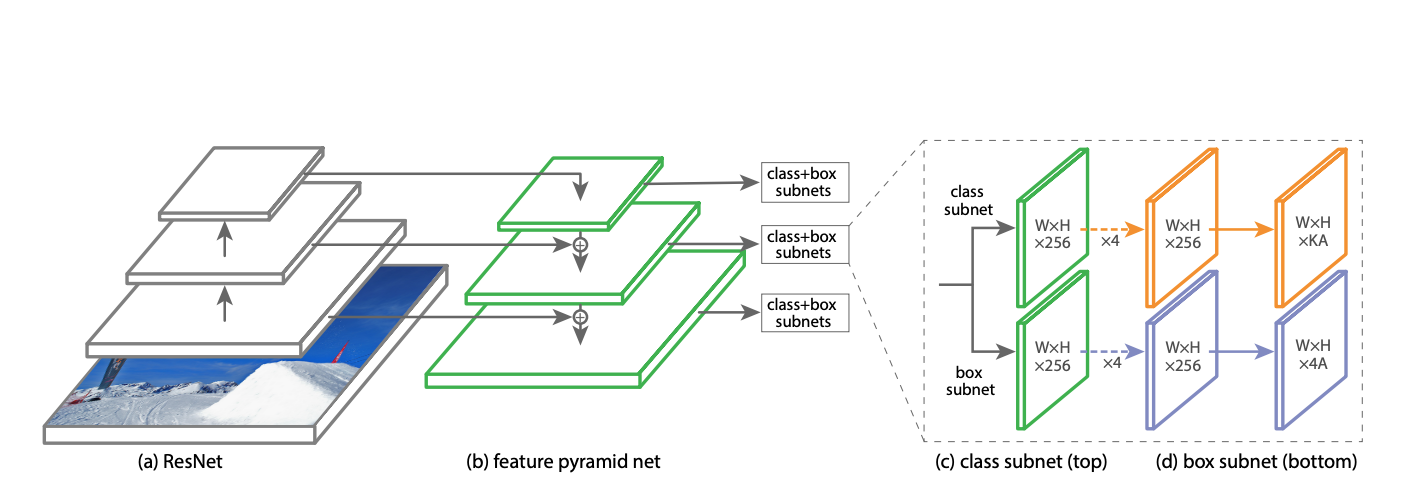
\includegraphics[scale = 0.36]{Figure/retinanet.png}
\caption{\footnotesize{RetinaNet architecture}}
\label{fig:retinanet}
\vspace{0mm}
\end{figure}
%%%%%%%%%%%%%%%%%%%%%%%%%%%%%%%%%%%%%%%%%%%%%%%%%%%%%

\noindent Focal loss is a loss function resembling cross entropy loss, but it is reshaped to down-weight easy example and focus training on hard negative samples. Feature Pyramid Network (FPN) is originally a two-stage detector providing both bottom-up and top-down pathways(Fig.~\ref{fig:retinanet}). Bottom-up pathway extracts features, and top-down pathway combines features with layers in bottom-up pathway. Classification sub-net predicts the probability of the presence of objects at a position and box regression sub-net computes the bounding box.\\

\noindent Compared to YOLOv3, RetinaNet has slightly higher prediction accuracy, but longer detection time.

\section{Experiments and Results}
This section shows the results of experiments and quantitative comparisons with other methods.\\

\noindent After applying YOLO, R-CNN and DPM on the VOC 2007, Picasso, and People-Art Datasets, the result shows that YOLO has the best performance(Fig.~\ref{fig:R_1}) in AP value which means it has better accuracy than the other two models.

%%%%%%%%%%%%%%%%%%%%%%%%%%%%%%%%%%%%%%%%%%%%%%%%%%%
\begin{figure}[ht]
\hspace{-10mm}
\centering
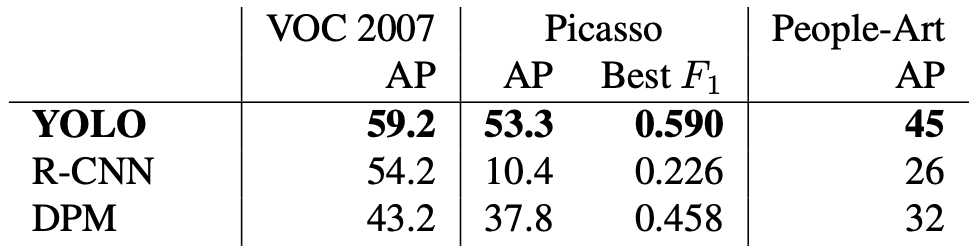
\includegraphics[scale = 0.4]{Figure/Results_1.png}
\caption{\footnotesize{Quantitative results on the VOC 2007, Picasso, and People-Art Datasets.\footnotemark}}
\label{fig:R_1}
\vspace{0mm}
\end{figure}\footnotetext{F1 score is a measure of a test's accuracy}
%%%%%%%%%%%%%%%%%%%%%%%%%%%%%%%%%%%%%%%%%%%%%%%%%%%%%
\noindent According to the result of applying Faster R-CNN, RetinaNet and YOLOv3 on MS CoCo Dataset, RetinaNet has the best accuracy (Fig.~\ref{fig:R_2}). However, viewed from inference time YOLOv3 is much faster than RetinaNet (Fig.~\ref{fig:R_3}).
%%%%%%%%%%%%%%%%%%%%%%%%%%%%%%%%%%%%%%%%%%%%%%%%%%%
\begin{figure}[ht]
\hspace{-10mm}
\centering
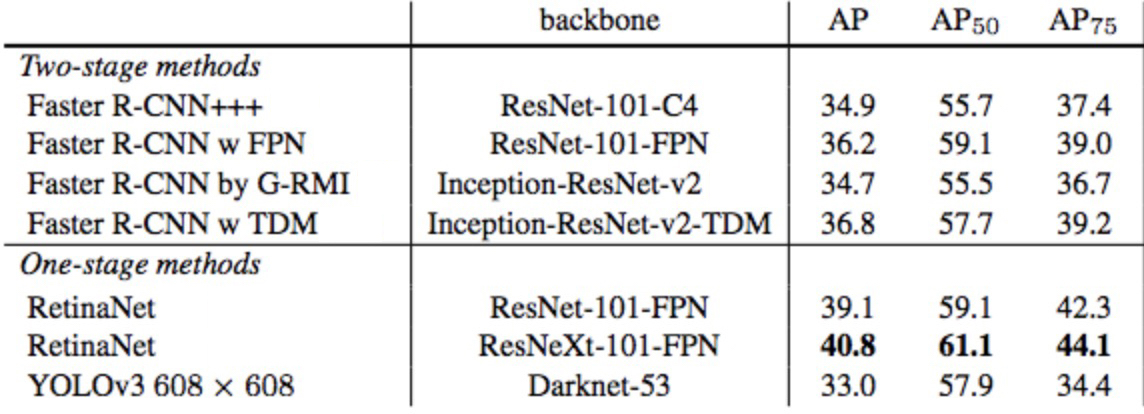
\includegraphics[scale = 0.2]{Figure/Result_2.jpg}
\caption{\footnotesize{Quantitative results on MS CoCo.}}
\label{fig:R_2}
\vspace{0mm}
\end{figure}
%%%%%%%%%%%%%%%%%%%%%%%%%%%%%%%%%%%%%%%%%%%%%%%%%%%
%%%%%%%%%%%%%%%%%%%%%%%%%%%%%%%%%%%%%%%%%%%%%%%%%%%
\begin{figure}[ht]
\hspace{-10mm}
\centering
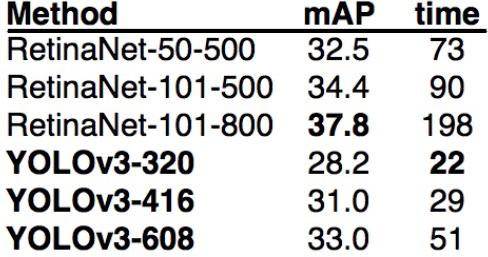
\includegraphics[scale = 0.5]{Figure/Result_3.jpg}
\caption{\footnotesize{Inference time on MS CoCo.}}
\label{fig:R_3}
\vspace{0mm}
\end{figure}
%%%%%%%%%%%%%%%%%%%%%%%%%%%%%%%%%%%%%%%%%%%%%%%%%%%

\subsection{Real-world Dataset}
Since our app mainly focuses on human object detection, we are keen to find some datasets that involve moving person objects and use them to train and test our algorithm specifically on top of the pre-trained model we have selected. Followed are some relevant real-world datasets that can be useful for training and testing:
\begin{itemize}
    \item Zero-Occlusion-Object-Tracking-Data-Set\footnote{https://github.com/csbuja/Zero-Occlusion-Object-Tracking-Data-Set}
    \item Scramble Crosswalks\footnote{http://data-lahub.opendata.arcgis.com/datasets/ladot::scramble-crosswalks}
    \item Help Blind Community to walk\footnote{https://www.kaggle.com/hamzafar/look4me}
    \item Run or Walk\footnote{https://www.kaggle.com/vmalyi/run-or-walk}
\end{itemize}

\section{Future Work}
In the future, \textit{Visionary} can be further developed to provide more reliable, accurate and complete services.\\

\noindent The framework should be further optimized for phone and achieve faster real-time output. Now, due to hardware constraints of the laptops, our demonstration still lags behind real-time performance. But a good existing example is app \textit{iDetection} available on Apple App Store. This app simply builds YOLOv3 on iPhone and it works with low latency. Ideally, \textit{Visionary} is expected to be developed to perform real-time tasks.\\ 

\noindent Currently, \textit{Visionary} outputs voice when bounding box size increases. But when a pedestrian is very far from the user, the voice guide should ignore the person even if he is approaching. To resolve this problem and offer a more complete solution, camera needs to take both RGB and depth information. With depth images, the distance from the user to the person can be retrieved and \textit{Visionary} won't warn the user when obstacle is far away. On Apple Store, a tool \textit{Depth Cam - Depth Editor} capturing depth images is found. Thus, we will integrate its functionality to \textit{Visionary}.



\newpage

\section{Appendix: Team work}
\subsection{Work Allocation}
\begin{table}[ht!]
\centering
\resizebox{1\linewidth}{!}
{
\begin{tabular}{|l|c|}
\hline
\textbf{Team Member} &  \textbf{Role}  \\ \hline
Jin Shuyuan &  Researched on YOLOv3 algorithm \\ 
    &  and set up project code\\
\hline
Mou Ziyang & Researched on other models \\ 
& and made comparison with YOLOv3\\ \hline
Tian Xin & Researched on DPM model \\
 & and compare their performance \\ \hline
Tian Xueyan & Researched on YOLOv3 algorithm \\ 
 & and datasets \\ \hline
Wang Tengda & Researched on other models \\
 & and made comparisons with YOLOv3 \\ \hline
Zhao Tianze & Applied model, developed bounding box \\
 & comparison algorithm and voice output feature\\ \hline
\end{tabular}
}
\vspace{-2mm}
\caption{\footnotesize{Team members' roles.}}
\label{tab:time}\vspace{-1em}
\end{table}

\subsection{Reflections}
\begin{itemize}
    \item {\textbf{Jin Shuyuan}}
After we started to look into the details of YOLOv3, I found that there are lots of fine-tuned parts and modifications in settings which really takes rigorous experiments and lots of experiences.
\item{\textbf{Mou Ziyang}}
It was very exciting to research on various machine learning models and try to understand their rationales. Although it was challenging, finding out how fast these models updated was very intriguing to me. After the project, I had a better overview of machine learning.
\item{\textbf{Tian Xin}}
Using machine learning models to solve real world problems is meaningful. During the process of this project, I gained a lot of knowledge about different object detection algorithms.
\item{\textbf{Tian Xueyan}}
The procedure of formulating a new problem, researching on various machine learning models and solving a problem using the chosen one is greatly rewarding for me. I was hence driven to look into details of YOLOv3 as well as other algorithms and I learned how to evaluate models and how to associate models with real-world problems.
\item{\textbf{Wang Tengda}}
It was a truly fruitful experience researching on various machine learning models, making comparisons and applying them to solve real-world problems. Frankly speaking, it was tough reading Through this project, I got exposed to state-of-the-art ML algorithms and had great fun working as a team 
\item{\textbf{Zhao Tianze}}
After we discussed about the different applications of machine learning, I noticed that machine learning could be widely used in different field. Compared with other algorithms, machine learning algorithm usually has a high accuracy result and could be optimized to an acceptable short time complexity. After I worked with the YOLOv3 model, I found that the input of this model is agile - it accept different resolution of images as input, also accept video and webcam. It also provided different weight for user to find the best balance between speed and accuracy. These features made the YOLOv3 model suitable for all kind of devices. It is possible to apply it in a portable light-weight device to serve visually handicapped better.
\end{itemize}

\bibliographystyle{aaai}
\bibliography{References.bib}
\end{document}
